\section{Background and Previous Work}
\label{sec:locvqa_locatt_background}

\gls{vqa} models are neural networks that answer natural language questions about an image~\cite{antol2015vqa,goyal2017making,hudson2019gqa,tan2019lxmert}. The capability of \gls{vqa} models to interpret natural language questions is of great appeal, as the range of possible questions that can be asked is vast and can differ from those used to train the models. This has led to many proposed \gls{vqa} models for medical applications in recent years~\cite{ImageCLEFVQA_Med2018,liu2019effective,liao2020aiml,vu2020question,zhan2020medical,gong2021cross,yu2023question}. These models can enable clinicians to probe the model with nuanced questions, thus helping to build confidence in its predictions.

Recent work on \gls{medvqa} has primarily focused on building more effective model architectures~\cite{gong2021cross,ren2020cgmvqa,vu2020question} or developing strategies to overcome limitations in \gls{medvqa} datasets~\cite{Nguyen19,liu2021slake,pelka2018radiology,do2021multiple,vu2020question}. Another emerging trend is to enhance \gls{vqa} performance by addressing the consistency of answers produced~\cite{tascon2022consistency}, particularly when considering entailment questions (\ie, the answer to ``Is the image that of a healthy subject?" should be consistent with the answer to ``Is there a fracture in the tibia?"). Despite these recent advances, however, most \gls{vqa} models are restricted to questions that consider the entire image at a time. Specifically, \gls{vqa} typically uses questions that address content within an image without specifying where this content may or may not be in the image. Yet the ability to ask specific questions about regions or locations of the image would be highly beneficial to any user as it would allow fine-grained questions and model probing. For instance, Fig.~\ref{fig:examples_data} illustrates examples of such \emph{localized questions} that combine content and spatial specifications. In the medical field, posing localized questions can significantly enhance the diagnostic process by providing second opinions to medical experts about suspicious regions. Additionally, this approach can improve trustworthiness by assessing the consistency between answers to both global and localized questions.

To this day, few works have addressed the ability to include location information in \gls{vqa} models. In~\cite{mani2020point}, localization information is posed in questions by constraining the spatial extent to a point within bounding boxes yielded by an object detector. The model then focuses its attention on objects close to this point. However, the method was developed for natural images and relies heavily on the object detector to limit the attention extent, making it difficult to scale in medical imaging applications. Alternatively, the approach from~\cite{vu2020question} answers questions about a pre-defined coarse grid of regions by directly including region information into the question (\eg, ``Is grasper in (0,0) to~(32,32)?"). This method relies on the ability of the model to learn a spatial mapping of the image and limits the regions to be on a fixed grid. Localized questions were also considered in~\cite{tascon2022consistency}, but the region of interest was cropped before being presented to the model, assuming that the surrounding context is irrelevant for answering this type of question.
\begin{figure}[!t]
\begin{center}
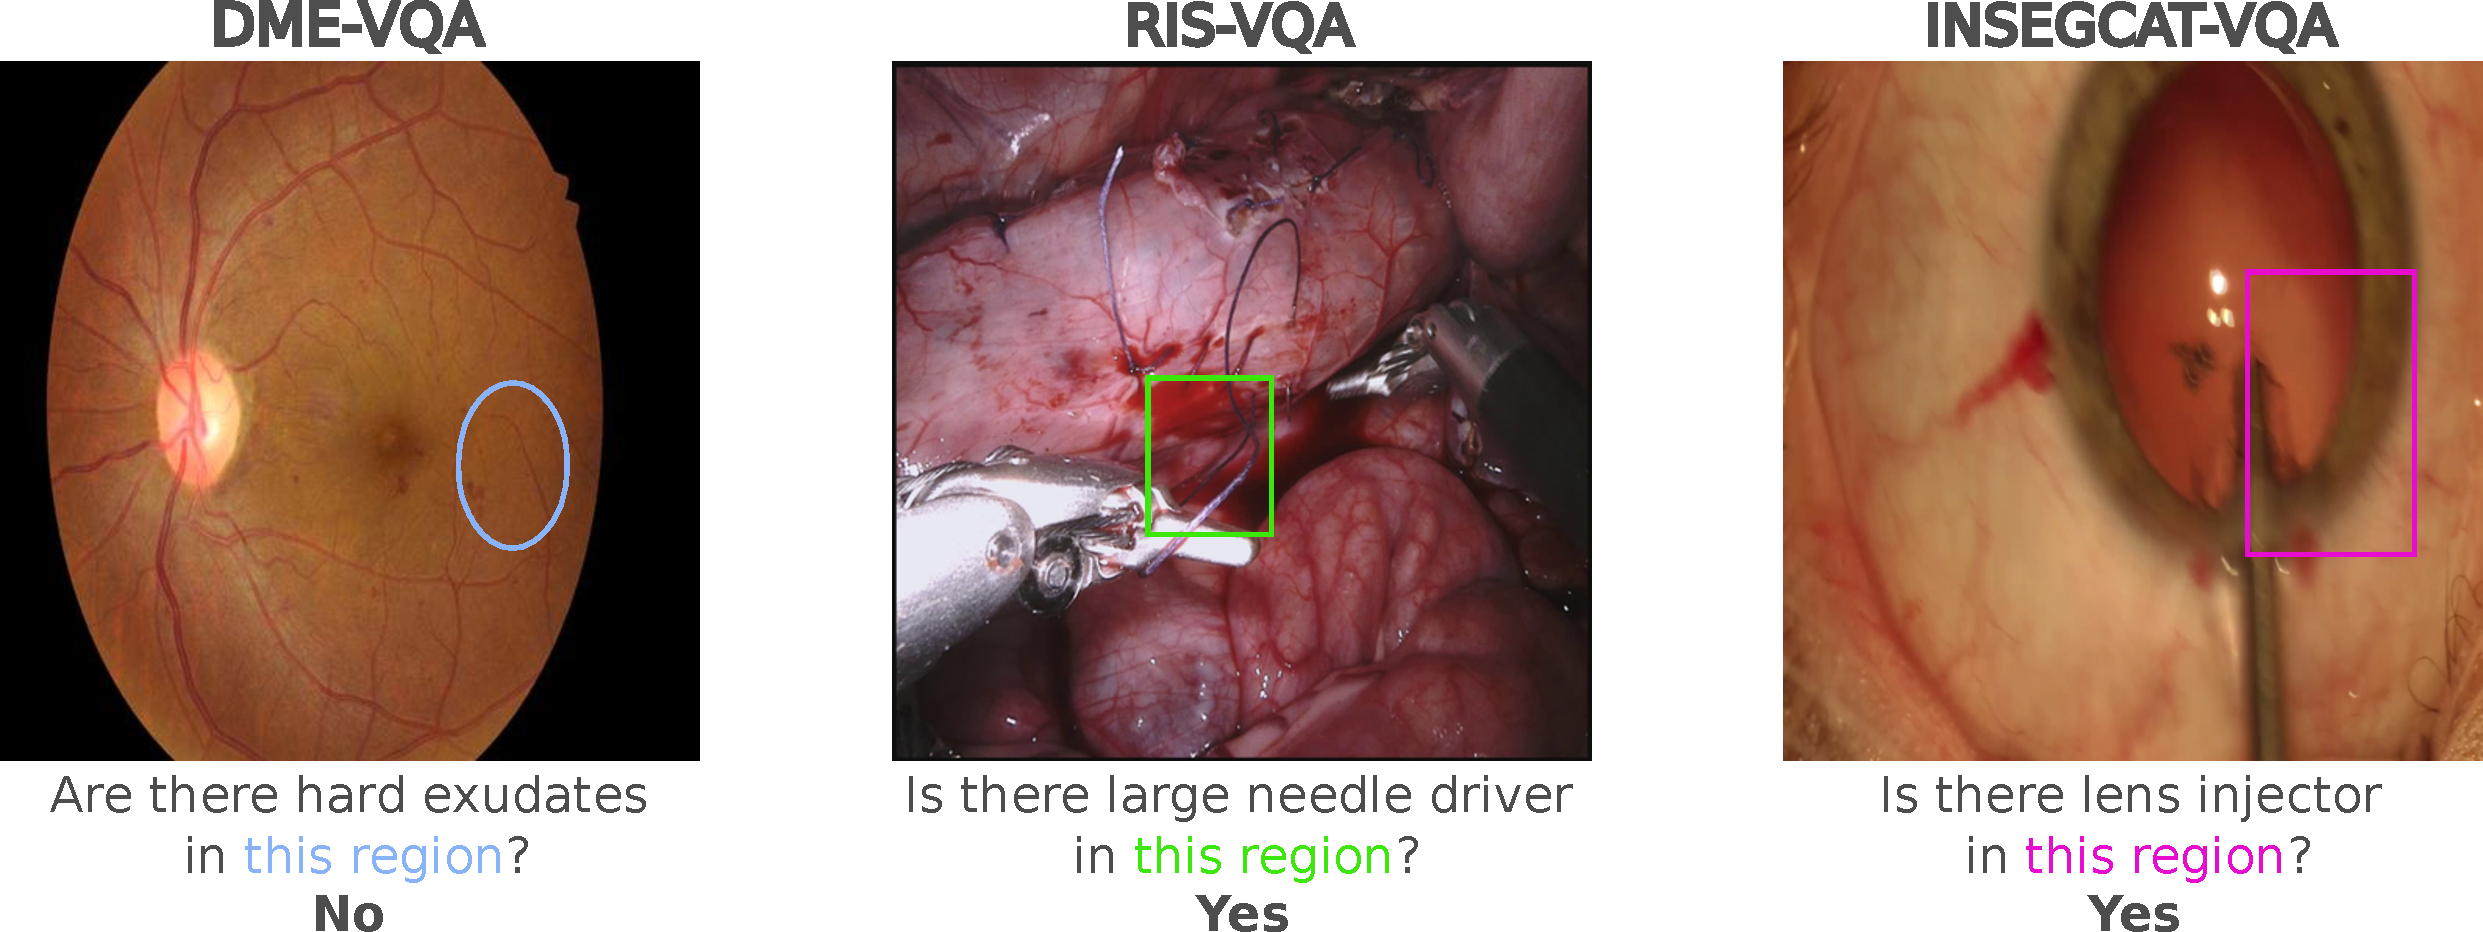
\includegraphics[width=0.9\textwidth]{Figures/Part1_LocVQA/01_locatt/examples_data.pdf}
\caption{Examples of localized questions. In some cases (RIS-VQA and INSEGCAT-VQA), the object mentioned in the question is only partially present in the region. We hypothesize that context can play an important role in answering such questions.}
\label{fig:examples_data}
\end{center}
\end{figure}

To overcome these limitations, we propose a novel \gls{vqa} architecture that alleviates the mentioned issues. At its core, we hypothesize that by allowing the \gls{vqa} model to access the entire images and properly encoding the region of interest, this model can be more effective at answering questions about regions. To achieve this, we propose using a multi-glimpse attention mechanism~\cite{ben2017mutan,vu2020question,tascon2022consistency} restricting its focus range to the region in question, but only after the model has considered the entire image. By doing so, we preserve contextual information about the question and its region. We evaluate the effectiveness of our approach by conducting extensive experiments on three datasets and comparing our method to state-of-the-art baselines. Our results demonstrate performance improvements across all datasets. 